\section{Experiments}
\label{sec:experiments}

%%%%%%%%%%%%%%%%%%%%%%%%%%%%%%%%%%%%%%%%%%%%%%%%%%%%%%%%%%%%
\begin{figure*}[t]
%%%%%%%%%%%%%%%%%%%%
\begin{minipage}[b]{0.29\linewidth}
               \centering
%%             \small
%              \begin{tabular}{l|rr|rr|}
%              (D10,                                                  T10)                                    & Naive                        (5M)                                     & Mahif                      (5M)                          & Naive                        (50M)                                          & Mahif                      (50M) \\ \cline{1-5}
%              U10                                                    & 125.587s                              & 8.145s                       & 1423.456s                              & 90.187s                    \\
%              U20                                                    & 121.911s                              & 8.467s                       & {\color{red}                           time                         out                           (30m)}                         & 90.513s                                      \\
%              U50                                                    & 277.642s                              & 10.448s                      & {\color{red}                           time                         out                           (30m)}                         & 84.611s                                      \\
%              U100                                                   & 502.570s                              & 18.761s                      & {\color{red}                           time                         out                           (30m)}                         & 116.525s                                     \\
%              U200                                                   & 1263.736s                             & 74.494s                      & {\color{red}                           time                         out                           (30m)}                         & 194.292s
%              \end{tabular}
               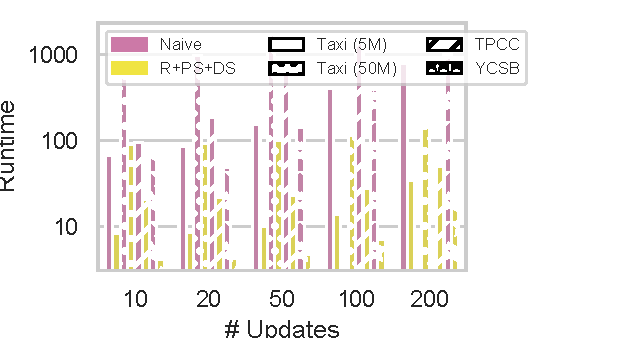
\includegraphics[width=1.1\linewidth,trim=0            0 0                                     0,                             clip]{imgs/felix_naive.pdf}              \\
               \vspace{-4mm}
               \caption{Naïve                                         vs.                                     Mahif                          (sec)}
               \label{fig:Naive                                       vs                                      Mahif}
               \end{minipage}
               %%%%%%%%%%%%%%%%%%%
%%%%%%%%%%%%%%%%%%%%
               \begin{minipage}[b]{0.35\linewidth}
               \centering
               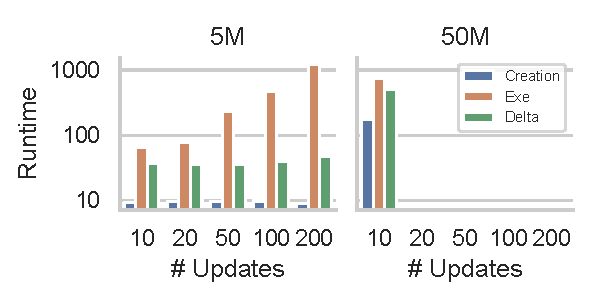
\includegraphics[width=0.95\linewidth,trim=0 8 0                                     0,                             clip]{imgs/felix_naive_breakdown.pdf}    \\
               \vspace{-3mm}
               \caption{Breakdown Naïve}
               \label{fig:Naive Method}
               \end{minipage}
%%%%%%%%%%%%%%%%%%%%
\begin{minipage}[b]{0.34\linewidth}
\centering
               % \scalebox{0.8}{
%              \scriptsize
%              \begin{tabular}{|r|rrrr|rrrr|}
%              \hline
%              & \multicolumn{4}{c|}{\textbf{5M}}                     & \multicolumn{4}{c|}{\textbf{50M}}     \\
%              \hline
%              \rotatebox{90}{\textbf{Updates}}                       & \rotatebox{90}{\textbf{PS}}           & \rotatebox{90}{\textbf{Exe}} & \rotatebox{90}{\textbf{R+PS+DS}}       & \rotatebox{90}{\textbf{R}} & \rotatebox{90}{\textbf{PS}} & \rotatebox{90}{\textbf{Exe}} & \rotatebox{90}{\textbf{R+PS+DS}$\,$$\,$$\,$} & \rotatebox{90}{\textbf{R}} \\
%              \hline
%              10                                                     & 0.07                                  & 8.08                         & 8.14                                   & 63.63                      & 0.07                        & 90.11                        & 90.18                                        & 722.23                     \\
%              20                                                     & 0.18                                  & 8.29                         & 8.47                                   & 81.12                      & 0.18                        & 90.33                        & 90.51                                        & 878.70                     \\
%              50                                                     & 1.30                                  & 9.15                         & 10.45                                  & 133.29                     & 1.29                        & 83.32                        & 84.61                                        & 1414.94                    \\
%              100                                                    & 8.46                                  & 18.76                        & 27.23                                  & 218.87                     & 8.46                        & 108.07                       & 116.53                                       & 2310.84                    \\
%              200                                                    & 62.13                                 & 12.36                        & 74.49                                  & 400.71                     & 62.22                       & 132.07                       & 194.29                                       & 4173.17                    \\
%              \hline
%              \end{tabular}
%              }
               \resizebox{1\linewidth}{!}{
               \begin{tabular}{|ll|rrrrr|}
               \hline
               &                                  &                   \multicolumn{5}{c|}{\textbf{\#Updates}} \\
               \textbf{Size}                                          & \textbf{Method}                       & \textbf{10}                  & \textbf{20}                            & \textbf{50}                & \textbf{100}                & \textbf{200}                 \\                                             \hline
               %
               \multirow{4}{*}{\textbf{5M}}                           & PS                                    & {{1}}                         & {{2}}                                   & {{3}}                       & {{4}}                        & {{5}}                        \\
               & Exe                                                  & {{6}}                                  & {{7}}                         & {{8}}                                   & {{9}}                      & {{10}}                       \\
               & R+PS+DS                                              & {{11}}                                  & {{12}}                         & {{13}}                                  & {{14}}                      & {{15}}                       \\
               & R                                                    & {{16}}                                 & {{17}}                        & {{18}}                                 & {{19}}                     & {{20}}                      \\                             \hline
               \multirow{4}{*}{\textbf{50M}}                          & PS                                    & {{21}}                         & {{22}}                                  & {{23}}                       & {{24}}                        & {{25}}                        \\
               & Exe                                                  & {{26}}                                 & {{27}}                        & {{28}}                                  & {{29}}                     & {{30}}                      \\
               & P+PS+DS                                              & {{31}}                                 & {{32}}                        & {{33}}                                  & {{34}}                     & {{35}}                      \\
               & R                                                    & {{36}}                                & {{37}}                       & {{38}}                                & {{39}}                    & {{40}}                     \\
               \hline
               \end{tabular}
               }                                                                                                                                                                                                                                                                                                               \\[-4mm]
               %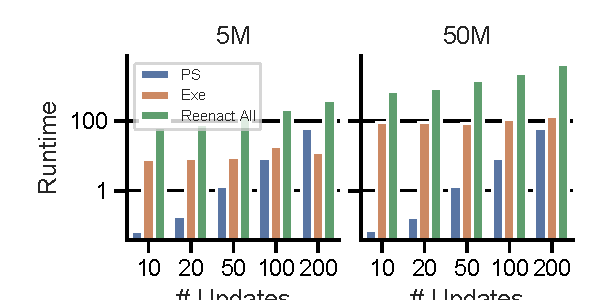
\includegraphics[width=0.95\linewidth,trim=0          0 0                                     0,                             clip]{imgs/felix_mahif_breakdown.pdf}    \\
               \caption{Breakdown                                     Mahif}
               \label{fig:Mahif                                       Method}
\end{minipage} \\
%%%%%%%%%%%%%%%%%%%%%
               \begin{minipage}[b]{0.245\linewidth}
               \centering
               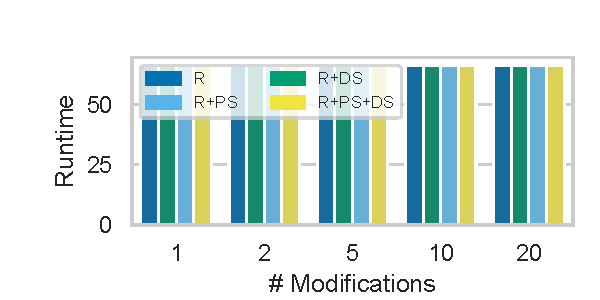
\includegraphics[width=0.95\linewidth,trim=7 5 0                                     0,                             clip]{imgs/felix_multimod.pdf}           \\
               \vspace{-3mm}
               \caption{Mult. Modifications}
               \label{fig:Multimod}
\end{minipage}
%%%%%%%%%%%%%%%%%%%%
\begin{minipage}[b]{0.275\linewidth}
               \hspace{-0.4cm}
               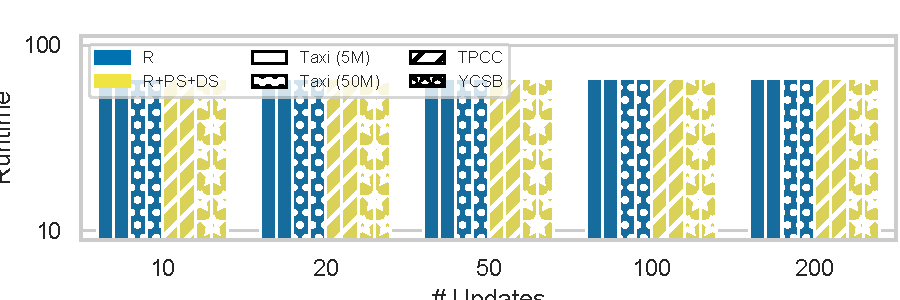
\includegraphics[width=1.2\linewidth,trim=0            0 0                                     0,                             clip]{imgs/felix_optimizations.pdf}      \\
               \vspace{-8mm}
               \caption{Optimization}
               \label{fig:optimization}
               \end{minipage}
%%%%%%%%%%%%%%%%%%%%%
               \begin{minipage}[b]{0.235\linewidth}
               \hspace{2mm}
               \scalebox{1}{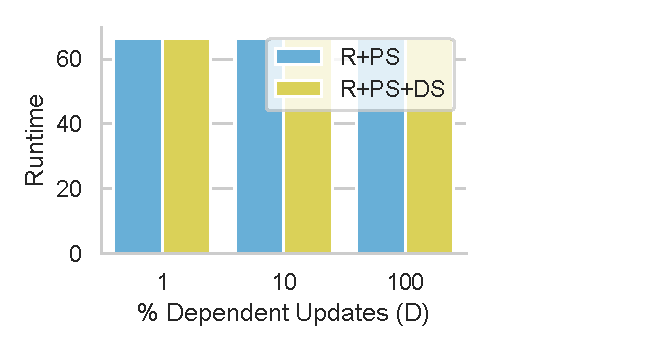
\includegraphics[width=1.0\linewidth,trim=22 0 50pt                                  0,                             clip]{imgs/felix_dependent_updates.pdf}} \\
               \vspace{-8mm}
               \caption{Dependent Updates}
               \label{fig:Dependent Updates}
               \end{minipage}
%%%%%%%%%%%%%%%%%%%%%
               \begin{minipage}[b]{0.225\linewidth}
               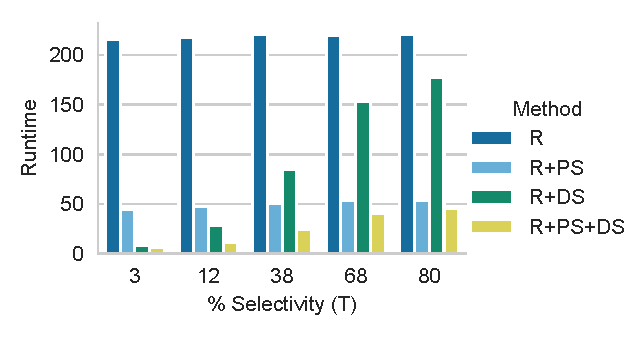
\includegraphics[width=1\linewidth,trim=0              0 0                                     0,                             clip]{imgs/felix_affected_data.pdf}      \\
               \vspace{-8mm}
               \caption{Affected                                      Data}
               \label{fig:Affected                                    Data}
               \end{minipage}                                         \\
%%%%%%%%%%%%%%%%%%%%
%              \begin{minipage}[b]{0.245\linewidth}
%              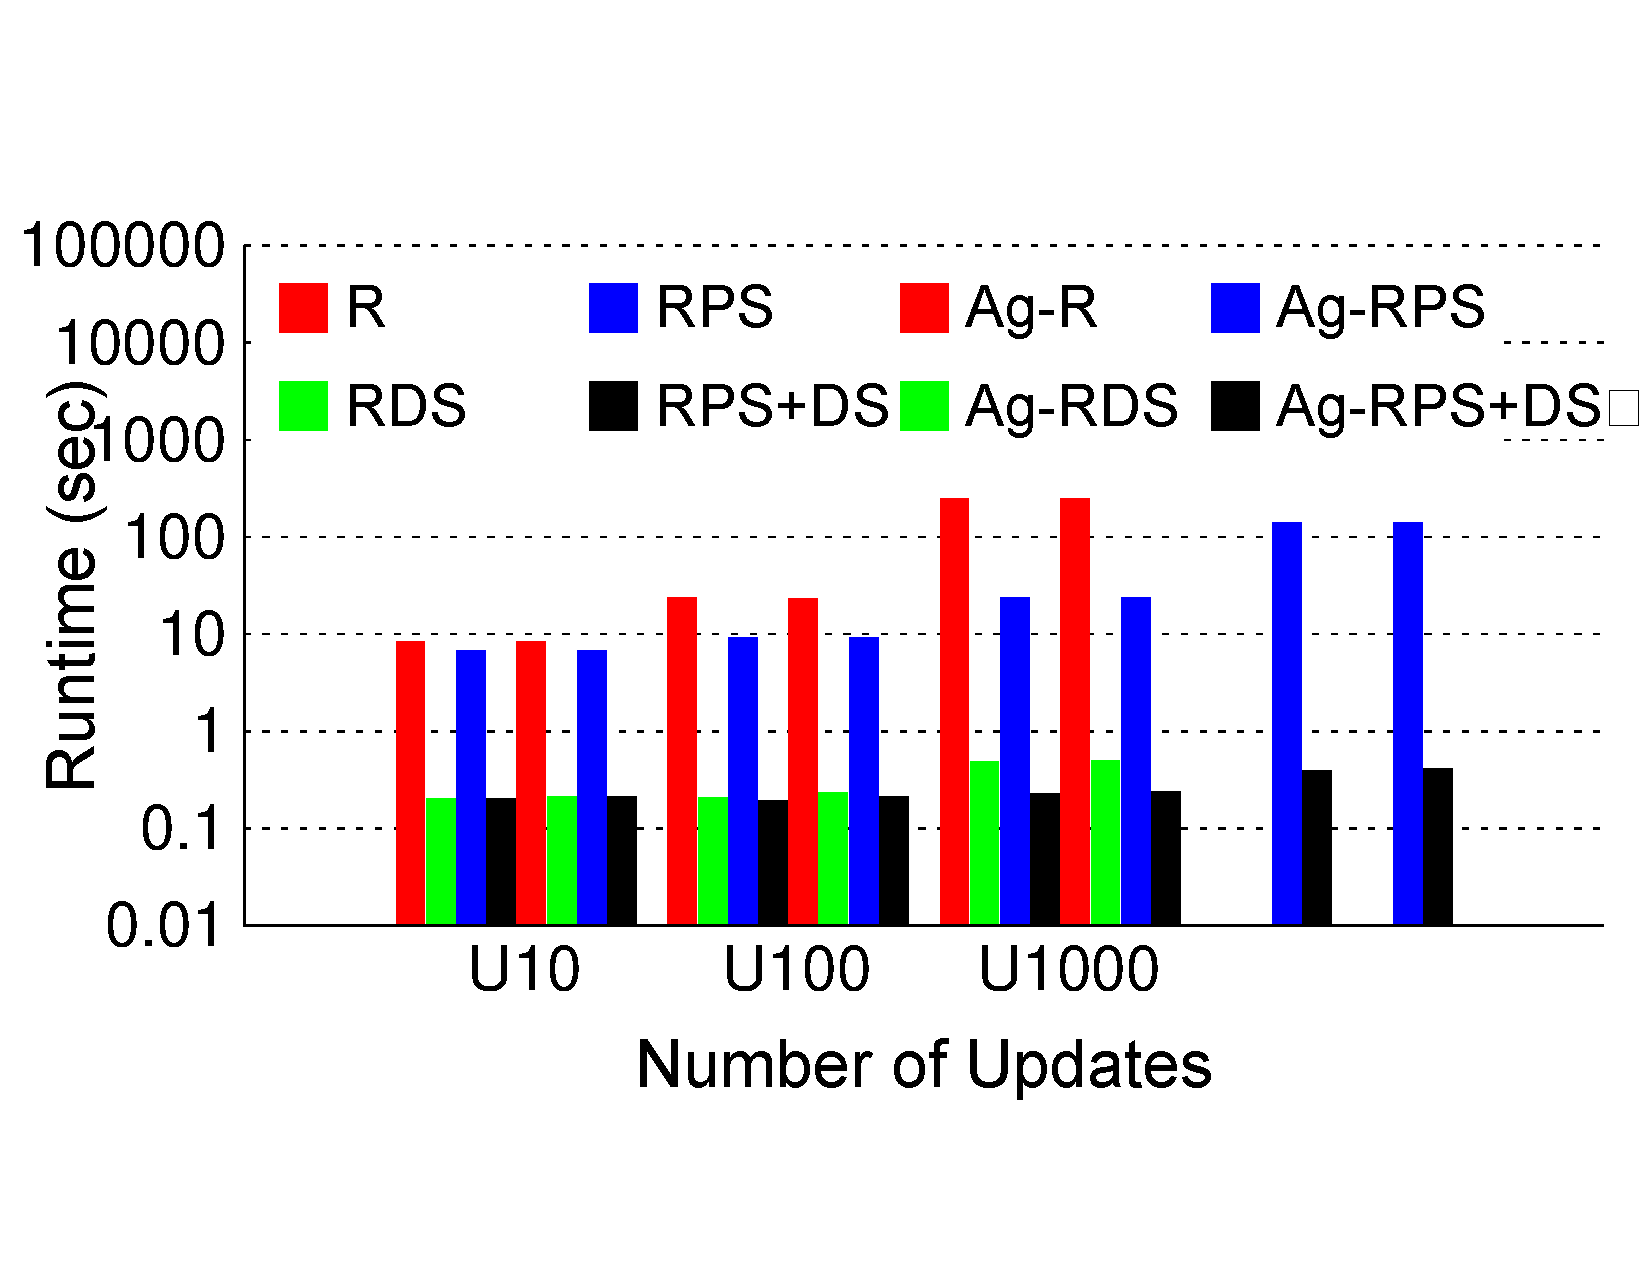
\includegraphics[width=1\linewidth,trim=0              50pt                                    0 80pt,                        clip]{imgs/aggregation.pdf}              \\
%              \vspace{-6mm}
%              \caption{Aggregation}
%              \label{fig:aggregation0}
%              \end{minipage}
%%%%%%%%%%%%%%%%%%%%%
\end{figure*}

%%% Local Variables:
%%% mode: latex
%%% TeX-master: "historical_whatif"
%%% End:


\newcommand{\mn}{\textit{N}\xspace}
\newcommand{\mr}{\textit{R}\xspace}
\newcommand{\mrd}{\textit{R+DS}\xspace}
\newcommand{\mrp}{\textit{R+PS}\xspace}
\newcommand{\mrdp}{\textit{R+PS+DS}\xspace}



We have conducted experiments to 1) evaluate the performance of our approach and compare it with the naïve approach, 2) examine the effectiveness of the proposed optimizations, and 3) study how our approach scales in database size and 
other important factors.
All experiments were performed on a machine with 2 x AMD Opteron 4238 CPUs (12 cores total), 128 GB RAM, and 4 x 1TB 7.2K
HDs in a hardware RAID 5 configuration. We used PostgreSQL 11.4 as the database backend.

Based on preliminary experiments, the variance of runtimes was determined to be low. We repeated each experiment at least 3 times and report average runtimes.


\subsection{Datasets and Workloads}\label{sec:exp-data-and-workloads}

\partitle{Datasets}
We use a taxi trips dataset from the Chicago's open data portal \footnote{https://data.cityofchicago.org/Transportation/Taxi-Trips/wrvz-psew (2020-10-13)}, as well as the standard TPC-C \footnote{TPC-C is an On-Line Transaction Processing Benchmark: http://www.tpc.org/tpcc/} and YCSB~\cite{CooperSTRS10} benchmarks to evaluate the performance of our approach. 
The original taxi dataset has $\sim100$M rows and 23 attributes.
The dataset contains trip information such as the \texttt{Company} (the taxi company), the \texttt{Taxi ID}, \texttt{Trip Start Timestamp}
(when the trip started), \texttt{Trip Seconds} (duration of the trip in seconds), \texttt{Trip Miles}
(distance of the trip in miles), \texttt{Pickup Community Area}, \texttt{Tips}, \texttt{Tolls}, \texttt{Extras} (tips, tolls and extra charges for the trip), and \texttt{Trip Total} (total cost of the trip).


We used samples from these tables amounting to 10\% ($5M$) and 50\% ($50M$) of the entire taxi dataset in some of the experiments. The TPC-C and YCSB benchmark databases were generated with OLTP-Bench \cite{DifallahPCC13}. For TPC-C, we used  the \texttt{stock} relation consisting of 10$M$ rows (scale factor 100).
 For YCSB database we used scale factor 5000, resulting in a single relation consisting of 5$M$ rows. The workloads generated by OLTP-Bench for each benchmark were modified to control the proportion of affected tuples.


\partitle{Workloads}

Unless stated otherwise, we use \abbrHWs with a single modification that modifies the first update in a history over a single relation.
We vary the following parameters. $U$ is the number of updates in the history (e.g. $U100$ for 100 updates). 
$M$ is the number of modifications made to the history.
$D$ is the percentage of updates that are dependent on the update(s) modified by the historical what-if query. We use 10\% as the default  ($D10$).

$T$ is the percentage of tuples in the relation that are affected by each dependent update (the default is 10\%), where $T0$ means that a small, constant number of tuples was affected. $I$ and $X$ are the percentage of statements in the history that are inserts and deletes, respectively.

Non-dependent statements affect a fixed fraction of the data equal to $T$, though independent from the tuples modified by dependent updates. 


\subsection{Compared Methods}
We compare the following methods in our experiments.
\textbf{Naïve (N)}: This method creates a copy of the database as of the start time of the history which is modified by the what-if query (\texttt{Creation}), executes $\deltaHist$ over this copy (\texttt{Exe}), and then computes the delta $\iDiff{\history(\db)}{\history[\deltaHist](\db)}$ by running a query over the current database state and the updated copy (\texttt{Delta}).
\textbf{Reenactment Only (R)} creates a reenactment query for $\history$ and for $\ahmod$.

We use run both reenactment queries over the database, and then compute the delta. \textbf{Reenactment with Data Slicing (R+DS)}: same as \mr except that we restrict reenactment to the part of data that is determined to be relevant  by our data slicing optimization. \textbf{Reenactment with Program Slicing (R+PS)}: same as the \mr method except that we only reenact the subset of updates from a slice determined by our program slicing optimization. \textbf{Reenactment with Program Slicing + Data Slicing (R+PS+DS)}:  we apply both optimizations.

\Cref{fig:Naive vs Mahif} shows the naïve method's performance in comparison to \mrdp. \Cref{fig:optimization} shows the runtime of reenactment (\mr) and reenactment with all optimizations enabled (\mrdp).  \Cref{fig:Mahif Method} breaks down the cost of \mrdp into \texttt{PS} and \texttt{Exe}, and together they form the runtime of \mrdp which should be compared to the cost of \mr (\texttt{Reenact All}). Given the clear efficiency gains of \mrdp over \mn and \mr, we omit \mn and \mr from most remaining experiments and focus on evaluating our optimizations.


%%%%%%%%%%%%%%%%%%%%%%%%%%%%%%%%%%%%%%%%%%%%%%%%%%%%%%%%%%%%
\begin{figure*}[t]
%%%%%%%%%%%%%%%%%%%%
\begin{minipage}[b]{0.48\linewidth}
    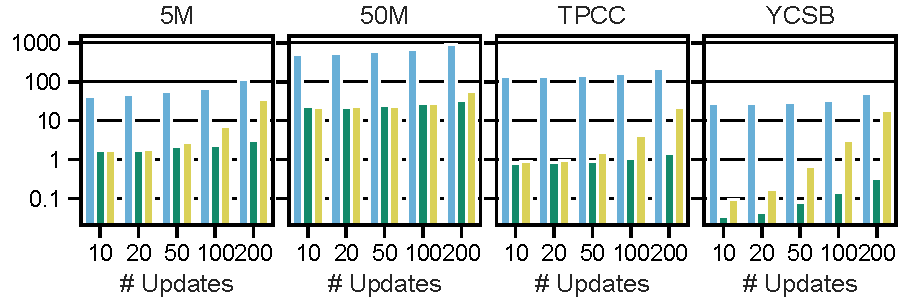
\includegraphics[width=1\linewidth,trim=0 0 0 0, clip]{imgs/felix_t0_optimizations.pdf}\\
    \vspace{-8mm}
  \caption{Datasets with T0}
  \label{fig:Relation Size}
  \end{minipage}
%%%%%%%%%%%%%%%%%%%%
 \begin{minipage}[b]{0.48\linewidth}
    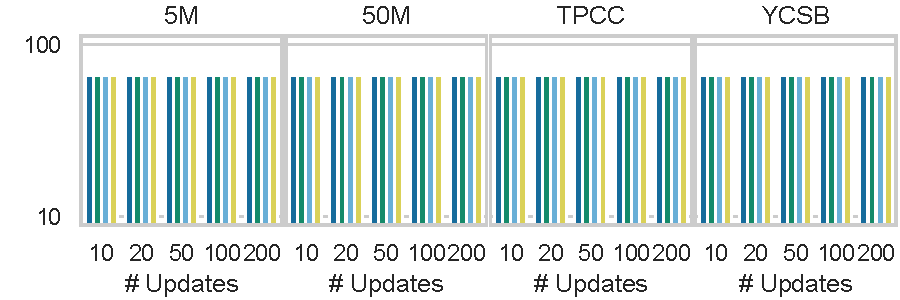
\includegraphics[width=1\linewidth,trim=0 0 0 0, clip]{imgs/felix_t10_optimizations.pdf}\\
    \vspace{-8mm}
  \caption{Datasets with T10}
  \label{fig:Relation Size1}
  \end{minipage}
  %%%%%%%%%%%%%%%%%%%%
\end{figure*}
\begin{figure}
  \begin{minipage}[b]{1\linewidth}
    $\,$\\[-5mm]
    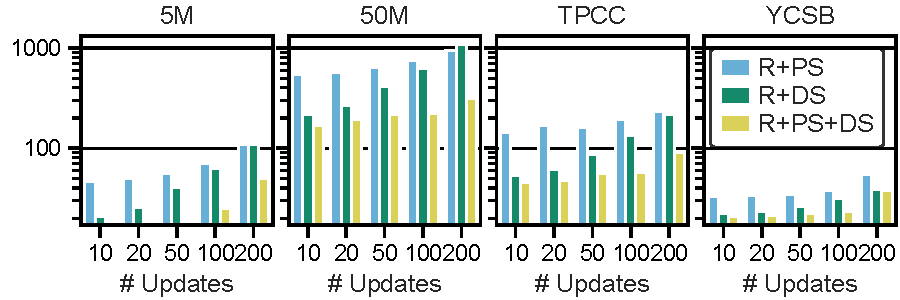
\includegraphics[width=1\linewidth,trim=0 0 0 0, clip]{imgs/felix_t25_optimizations.pdf}\\
    \vspace{-8mm}
  \caption{Datasets with T25}
  \label{fig:Relation Size2}
  \end{minipage}
%%%%%%%%%%%%%%%%%%%%
% %%%%%%%%%%%%%%%%%%%%%%%%%%%%%%%%%%%%%%%%
%% \begin{minipage}[b]{0.245\linewidth}
%%    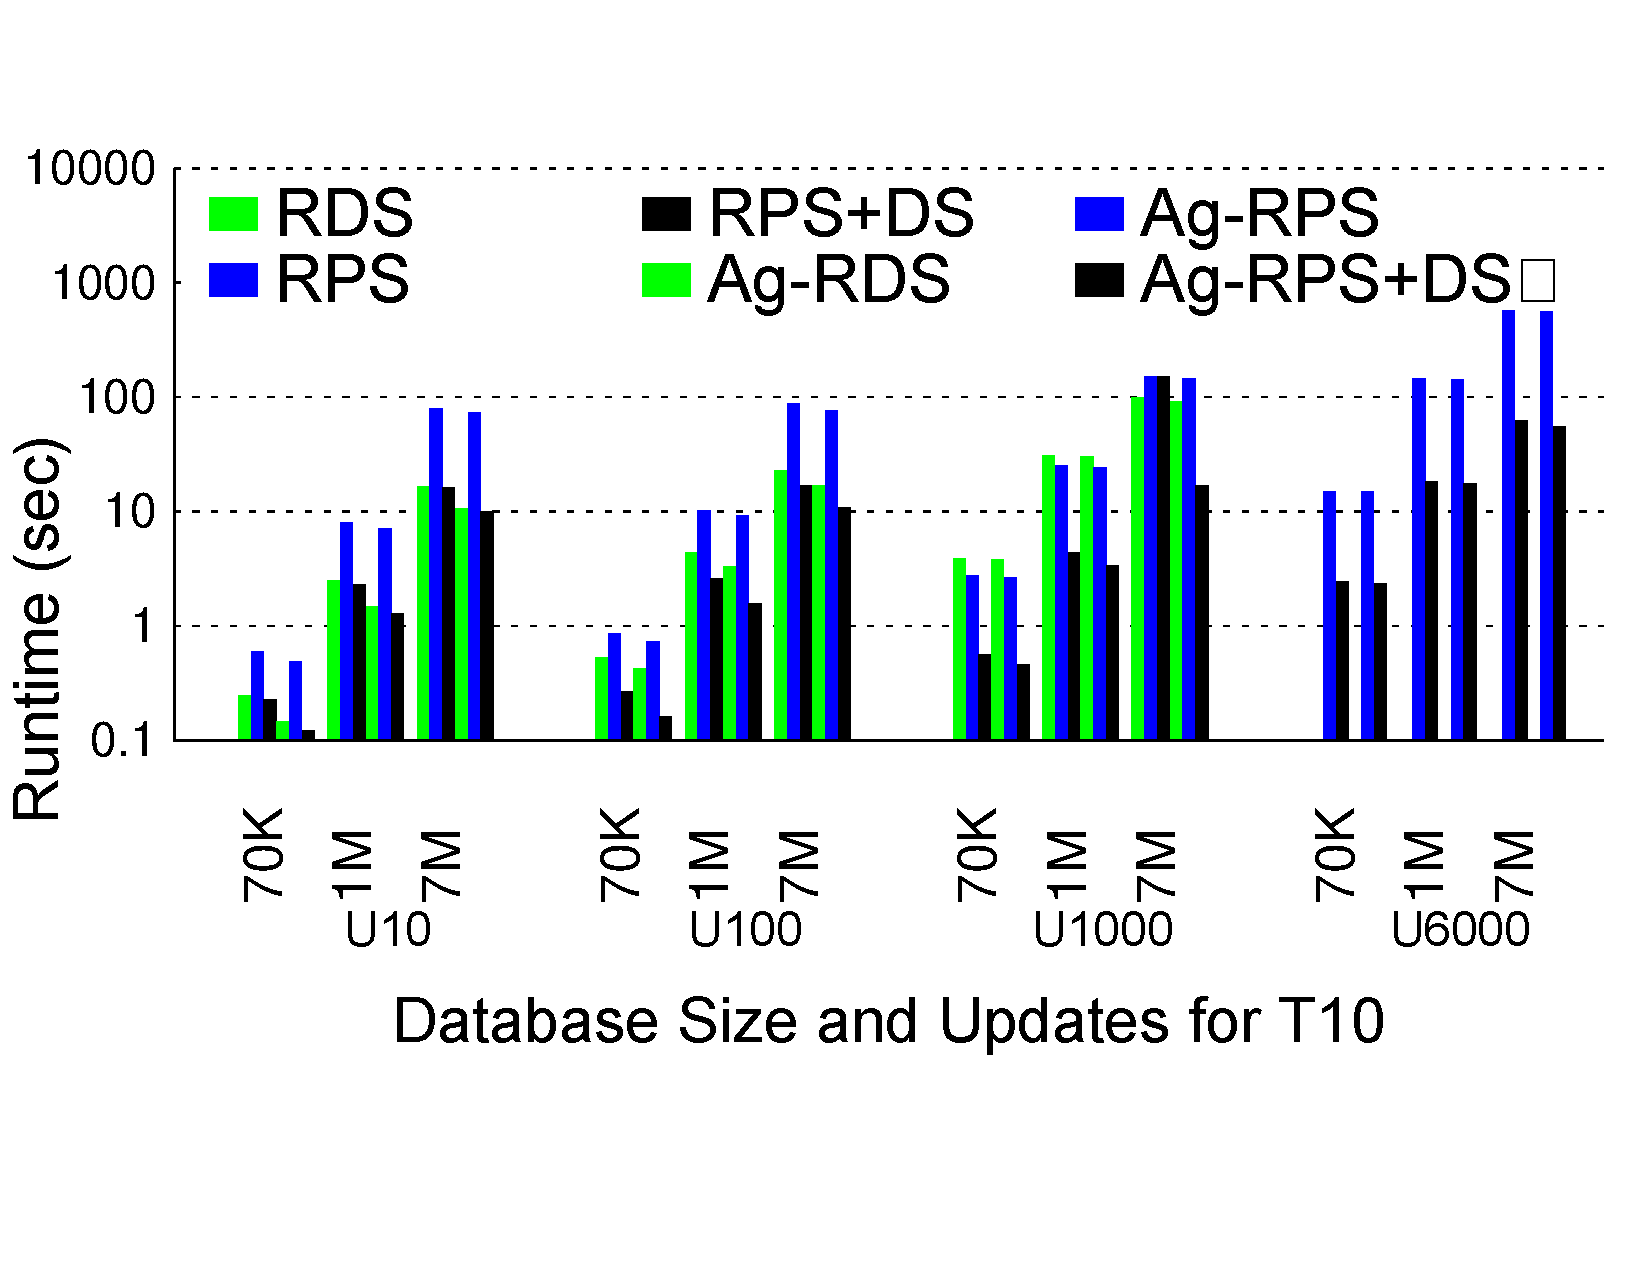
\includegraphics[width=1\linewidth,trim=0 50pt 0 80pt, clip]{imgs/agg10.pdf}\\
%%  \vspace{-6mm}
%%  \caption{Aggregate Query}
%%  \label{fig:aggregation0}
%%  \end{minipage}\\
%%%%%%%%%%%%%%%%%%%%
%   \begin{minipage}[b]{0.245\linewidth}
%    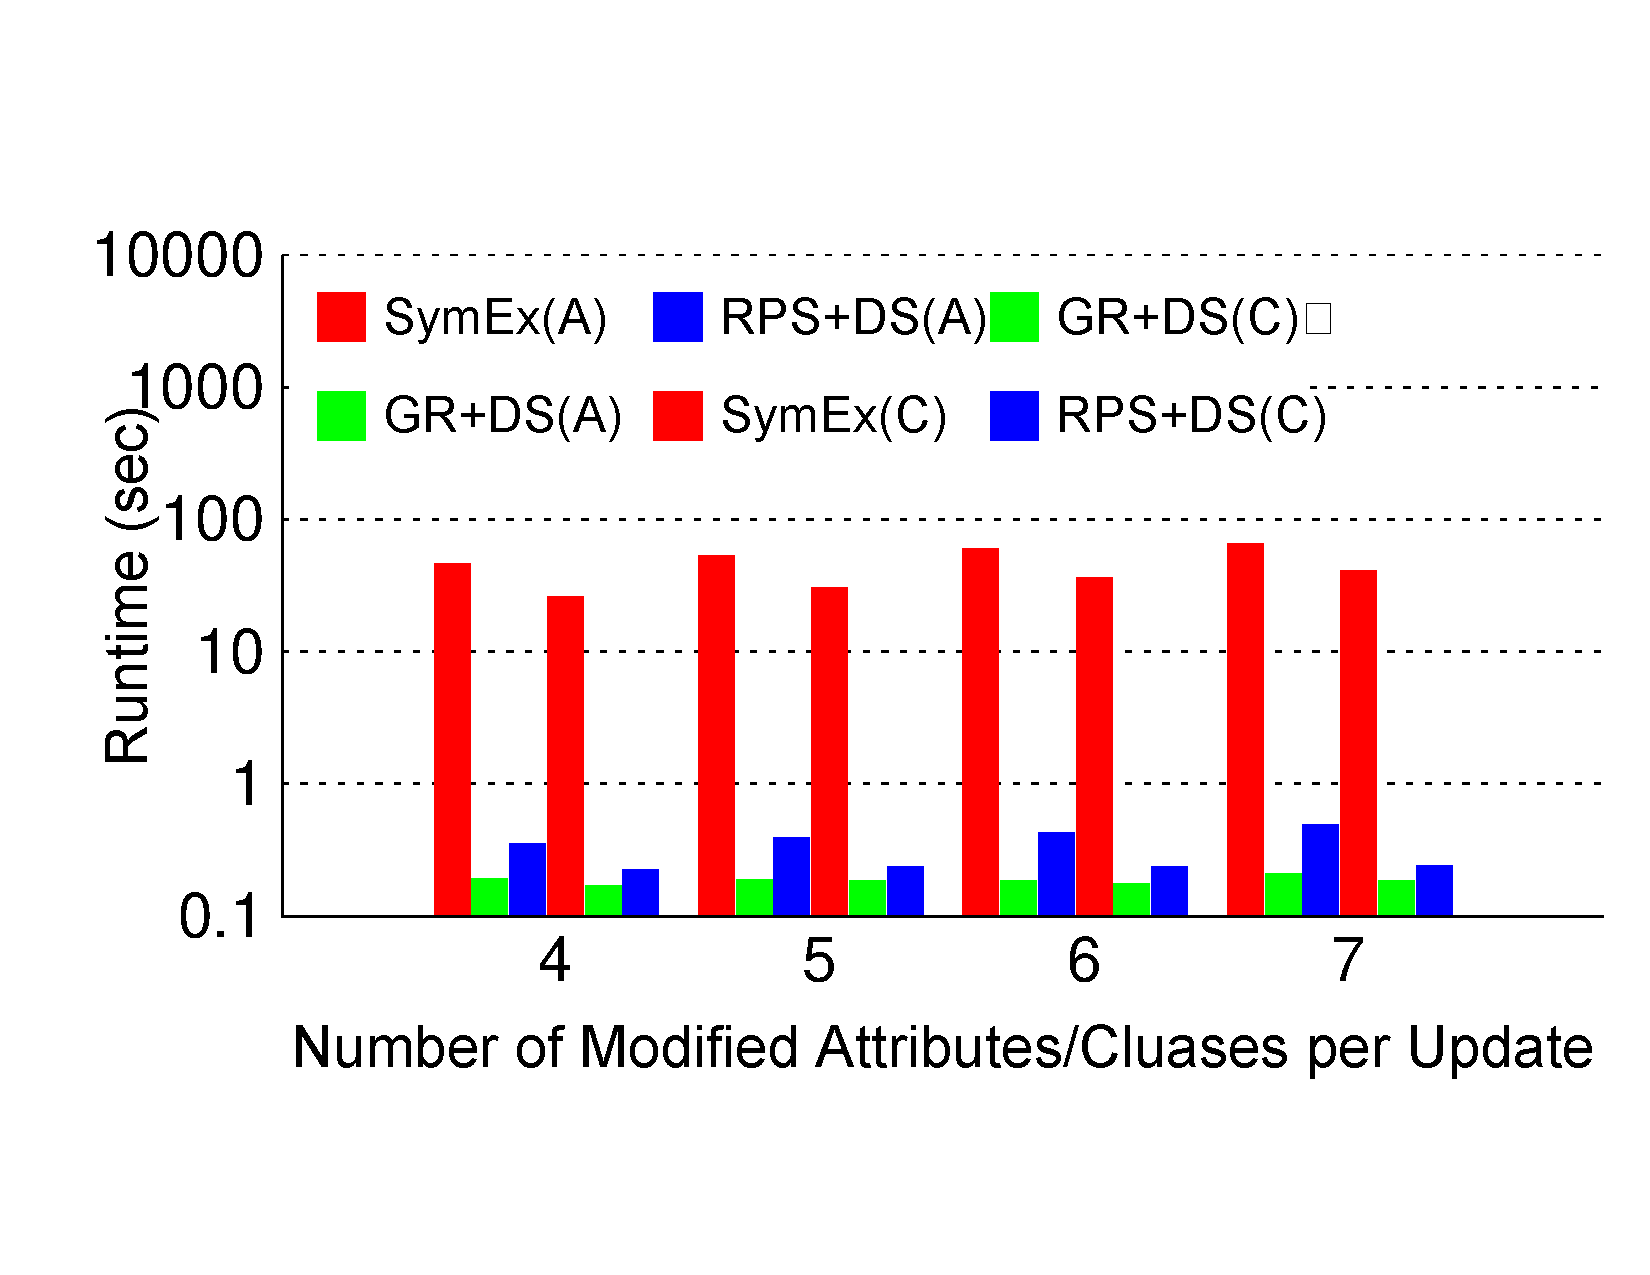
\includegraphics[width=1\linewidth,trim=0 50pt 0 80pt, clip]{imgs/attCla.pdf}\\
%  \vspace{-6mm}
%  \caption{Number of Attributes/Conditions}
%  \label{fig:Different Number of Attributes/Conditions}
%  \end{minipage}
%%%%%%%%%%%%%%%%%%%%
\end{figure}


%%% Local Variables:
%%% mode: latex
%%% TeX-master: "historical_whatif"
%%% End:





\subsection{Optimization Methods}
We now evaluate our optimization techniques varying the parameters introduced in \Cref{sec:exp-data-and-workloads} over update-only workloads to observe which workload characteristics benefit which optimization.

\partitle{Varying Datasets (at D10)} 
We vary number of updates and amount of tuples affected per update ($T0$, $T10$, $T25$). Overall, we see that our approach scales very well in dataset size. As the cost of program slicing is independent of the database size, larger datasets benefit much more from program slicing. 
For lower selectivity (\Cref{fig:Relation Size}), we see that \mrd is very competitive with \mrdp for the smaller Taxi dataset (5M) as reenactment of the entire history over a small relation and an even smaller proportion of affected input data is cheaper than the cost of solving the MILP problem for program slicing. Notably, for the YCSB dataset, the MILP cost exceeds the cost of $\mrd$, as data slicing is well-served by the physical correlation of the key used to update the data. For larger proportions of data to be reenacted (\Cref{fig:Relation Size1} and \Cref{fig:Relation Size2}),  \mrdp  consistently outperforms \mrp and \mrd. The optimal case for \mrdp is when the size of the  affected input data as determined by data slicing is large enough that calculating and reenacting over a slice is worth the execution cost of the generated MILP.

\partitle{Varying Percentage of Dependent Updates (at T10)}

\label{sec:exp-dep}

\Cref{fig:Dependent Updates} demonstrates the effect the proportion of dependent updates ($D$) in a given history has on \mrp, and how the addition of data slicing (\mrdp) is an effective way to mitigate these effects. This experiment uses the $5M$ row taxi trip table, with defaults T10 (10\% of tuples affected by modified updates) and U100 (100 updates in the history). As the proportion of dependent updates in the history increases, program slicing becomes less effective as more updates have to be included in the slice over the history. At D100 (100\% of updates are dependent), program slicing is not beneficial at all, but still incurs the MILP solver cost. However, data slicing  mitigates this effect, as the input to reenactment is filtered to include only a fraction of the data, making it more effective than \mrp at D100.


\partitle{Varying Affected Data (at U100, D1)}
\label{sec:exp-ds}
The effect of the percentage of  tuples affected by the updates modified by the \abbrHW ($T$) is examined in \Cref{fig:Affected Data}. This experiment is executed for 100 updates on the taxi trips relation with $5M$ rows. For example, $T3$ means 3\% of tuples ($\sim150$K out of 5M) are modified by the \abbrHW. The result demonstrates that varying $T$ does not change the performance of \mrp, as the whole history is evaluated over the full input table in all cases. However, increasing $T$, increases the runtime of \mrd and \mrdp considerably as data slicing becomes less efficient due to the greater amount of input data that needs to be accessed during reenactment. However, at moderate selectivity (T68), \mrdp provides enough filtering over the history and data to be more performant than either optimization alone. 

\subsection{Mixed Workloads with Deletes and Inserts}\label{sec:mixed-workl-updat}


\begin{figure}[t]
  \begin{minipage}[b]{0.47\linewidth}
    \centering
		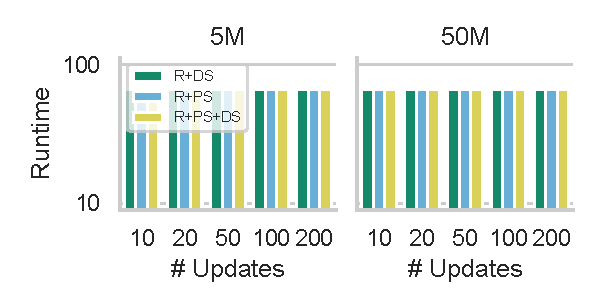
\includegraphics[width=1.1\linewidth,trim=10 9 15 10, clip]{imgs/felix_inserts.pdf}
		\vspace{-6.5mm}
		\caption{Inserts: I10, T10}
		\label{fig:Inserts at I10}
	\end{minipage}
	
	\begin{minipage}[b]{0.52\linewidth}
      \centering
      \hspace{3mm}
      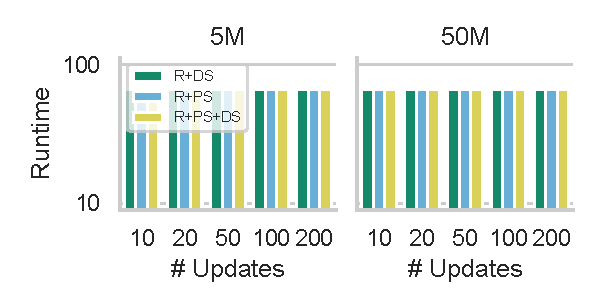
\includegraphics[width=0.9\linewidth,trim=30 9 15 10, clip]{imgs/felix_mixed.pdf}
		\vspace{-2.5mm}
		\caption{Mixed: I10, X10, T10}
		\label{fig:Mixed Updates at IX10}
	\end{minipage}
\end{figure}


We now consider workloads that contain deletions, inserts, and updates. Since deletes are handled in a similar fashion to updates, we mainly focus on evaluating the impact of the fraction of inserts on performance. We use the taxi trip tables for this experiment. 

As shown in \Cref{fig:Mixed Updates at IX10}, \mrdp outperforms the other methods for mixed workloads. When comparing to similar workloads presented in \Crefrange{fig:Relation Size}{fig:Relation Size2}, we see that introducing deletes and inserts into our workload in lieu of updates reduces the cost of reenactment and our optimizations. Note that delete statements result in fewer constraints in the program slicing MILP than update statements. Inserts are much cheaper to process than program slicing an update as we are able to reenact the unsliced prefix of the history on a very small amount of tuples (only the tuples being inserted, typically a very small fraction of a given workload).


\subsection{Varying the number of modifications}\label{sec:vary-numb-modif}
So far we have evaluated \abbrHWs with a single modification. We now evaluate how multiple modifications affect the performance of Mahif and of the proposed optimizations.

\Cref{fig:Multimod} depicts the effect of changing the number of modifications per \abbrHW. Program slicing is more expensive than its single modification counterpart, given that we have to test each update by comparing the state of its symbolic tuple not only between $\history$ and $\ahmod$, but duplicating these histories while removing the update being tested, in order to not falsely classify an update as independent. This effectively quadruples the individual MILP program size over the single modification case. Data slicing also becomes more expensive as we employ the push down technique described in \Cref{sec:filter}, which in turn creates a selection operator with a  larger, more complicated condition. Recall that such selection conditions basically include some partial reenactment in order to capture every tuple that would be modified by modifications that occur after the first modification in the \abbrHW. That is, program slicing and data slicing are less efficient for multiple modifications.

The data from \Cref{fig:Multimod} shows a decrease in performance from a single modification to the multiple modification case. The nature of the modification (attributes updated, conditions, selectivity, dependencies across updates) significantly impacts the performance of \mrd, as evaluating the data slicing conditions pushed down through a long history is sometimes expensive. \mrdp remains an effective optimization compared to \mr, though its cost is higher than for single modifications. In part this is due to the effect of slicing the history which also reduces the size of conditions produced by pushing down  data slicing conditions. It should be noted that as the amount of modifications grows, the program slicing time goes down as these modifications are inherently dependent. That being said, an inflection point is possible where the gains in program slicing execution speedup results in a slowdown from the longer history the data slicing conditions need to be pushed through.

\subsection{Summary}
Our approach outperforms the naïve method in most cases despite it not needing any additional storage. Even reenactment without optimizations is already considerably faster than the naïve method.
The proposed optimizations are very effective, especially for large number of updates and larger databases. However, for small relations or very low selectivity, the cost of program slicing will outweigh the cost of reenactment or reenactment with data slicing. Data slicing is very effective for single modifications, but less so for multiple modifications, because the size and complexity of the data slicing conditions increases when these conditions are pushed through the updates upstream from a modification. Our experiments also show that our approach scales well with respect to database size.

%%% Local Variables:
%%% mode: latex
%%% TeX-master: "historical_whatif"
%%% End: